\chapter{Extensiones Autoadjuntas del Operador}

	En este capítulo se va a estudiar otras posibles condiciones de contorno en $x=0$, que hacen que el operador sea hermítico. Luego se va a estudiar si admite extenciones autoadjuntas, y una vez obtenida se va a estudiar la nueva estructura de polos. 


\section{Condiciones de Contorno Regulares:}

En el capitulo anterior se estudiaron condiciones de contorno Dirichlet en ambos extremos, el objetivo de esta seccíon es ver si existen otras posibles condiciones de contorno.\\

Imponiendo las condiciones de contorno Robin mas generales, el operador queda definido por:

\begin{equation}
\begin{array}{c}
    A \phi (x) = - \partial ^2 _x  \phi(x) + \frac{\alpha}{x} \phi(x) \\
    \phi(L) = 0 \\
    \phi (0) + C \phi'(0) = 0 
\end{array}
\label{operador}
\end{equation}



En el capítulo 3 se mostró que las soluciones vienen dadas por:

\begin{equation}
    \phi (x) = 
    C[1]
    \underbrace{
     \ e ^{-i \lambda x} \ x \ F _{1} ^{1} (1+\frac{ \alpha}{2 \lambda i },2,2 i \lambda x) } _ {y_1}
    + C[2] \underbrace{ \ e^{-i \lambda x } \ x \ U (1+\frac{ \alpha}{2 \lambda i },2,2 i \lambda x) } _{y_2} 
\tag{\ref{eq.phi}}
\end{equation}

Donde el comportamiento a $x \rightarrow 0$ está calculado en (\ref{eq.scat}).

\begin{equation}
\begin{array}{c}
\phi (x \rightarrow 0) \approx
C[1] ( x + O(x ^2)) + \\[10pt]
C[2] x 
\left( 
\frac{1}{  \alpha x  \Gamma ( \frac{ \alpha}{2 i \lambda}  )   }  +
\frac{Log(x) }{\Gamma ( \frac{ \alpha}{2 i \lambda} ) } + Cte + O(x)
\right)
\end{array}
\tag{\ref{eq.scat}}
\end{equation}

Aquí puede verse que $y' (x \rightarrow 0 ) \approx  \frac{ Log (x) }{\Gamma \left( \frac{\alpha}{2 i \lambda}\right)} $, por lo tanto cuaquier condicion de contorno de la forma ( \label{eq.phi} ) va a implicar $C[2] = 0$.
 
Por lo tanto las únicas condiciones de contorno validas en $x=0$ son Dirichlet,  entonces el espectro está dado por los ceros de $y(L)$ o $y'(L)$. \\



En la proxima seccion, se van a  buscar extenciones autoajuntas de forma que pueda contener a $U(L)$ en el espectro.


\section{Artesanal:}

Dado el operador $A = - \partial ^2 _x + \frac{\alpha}{x}  $ se van a buscar las condiciones de contorno en $x=0$ que lo hagan autoadjunto.\\

La primer condicion necesaria es que su dominio e imagen pertenezcan a $L _2$.

\begin{equation}
\begin{array}{c}
si \ \phi \in L _2 \rightarrow A \phi \in L _2
\end{array}
\label{cond}
\end{equation}


Como $\phi (x)$ es bien comportada en el intervalo $(0,L]$, va a ser suficiente la integrabilidad en $x=0$ para que se cumpla (\ref{cond}). \\


La aplicación de $A$ sobre $y _1 (x \rightarrow 0)$ está dada por:


\begin{equation}
\begin{array}{c}
y _1 (x \rightarrow 0) \approx x + a _2 x ^2 + O (x ^3 ) \ \rightarrow y _2 \ \in \ L _2 \\
A y _2 (x \rightarrow 0) \approx \alpha - 2 a_2 + O(x ) \rightarrow y _1\in L _2
\end{array}
\label{eq.chico1}
\end{equation}

Esto tambien vale para cualquier potencia positiva mayor 1, no vale para funciones que van a una constante debido a que el termino $1/x$ lo vuelve no integrable en el origen, luego se estudiara mas formalmente esta afirmacion.

Visto el comportamiento de la segunda autofuncion, propongo su comportamiento en $x \rightarrow 0 $ sea :

\begin{equation}
\begin{array}{c}
\phi _2 (x \rightarrow 0) \approx 1 + \alpha x Log[x] \\
\mathscr{H} [\phi _2] (x \rightarrow 0 ) \approx \alpha ^2 Log[x] \ \in L _2
\end{array}
\label{eq.chico2}
\end{equation}

Con estas propuestas dos funciones cualquiera en el dominio del operador tienen el desarrollo a $x \rightarrow 0$ :

\begin{equation}
\phi , \chi = \beta , \beta _1 \ x + \gamma , \gamma _1 \ (1+ \alpha x Log[x] )
\label{eq.phi.chi}
\end{equation}

La siguiente condicion es pedir que operador sea simetrico.

\begin{equation}
(\phi, \mathscr{H} \chi ) = ( \mathscr{H} \phi , \chi )
\end{equation}

Para ello voy a pedir que se anulen los terminos de borde

\begin{equation}
\begin{array}{c}
\int _0 ^{L} 
\left(
- \partial ^2 _x + \frac{\alpha}{x}
\right)
\phi ^{*} \chi dx = \\
\phi ^{*'} \chi - \phi \chi ^{* '} + 
\int _0 ^{L} 
\phi ^{*} 
| _{x=0} ^{x=L}
\left(
- \partial _x ^2 + \frac{\alpha}{x}
\right)
\chi dx 
\end{array}
\end{equation}

Suponiendo que $\phi $ y $ \chi $ ya satisfacen la condicion de contorno en $x=L$ e insertando el desarrollo de $\phi$ y $\chi$ dado por ( \ref{eq.phi.chi} ) , obtengo que para que el termino de borde se satisfaga debe cumplirse:

\begin{equation}
\left(
-1 + \alpha x 
\right)
\left(
\beta _1 ^{* '} \gamma - \beta \gamma _1 ^{* '}
\right)
\end{equation}

La cual se satiface si se cumple la doncidion 

\begin{equation}
\gamma = c \beta 
\end{equation}

Entonces toda funcion que esté en el dominio del operador va a tener un desarollo dado por:

\begin{equation}
\phi ( x \rightarrow 0 ) \approx x + c \left(  1 + \alpha x Log[x]   \right)
\end{equation}

Para cada $c$ que yo elija voy a obtener un Hamiltoniano con unas condiciones de contorno que lo vuelvan autoadjunto

\section{Teoria de Von Neumann}


Dado un operador diferencial de segundo orden $\mathscr{H}$ hay que definir cieras condiciones de contorno para que sea Hermitico.

Una forma de encontrar las condiciones de contorno que hacen que un operador sea hermitico (en el caso que estamos estudiando) es que las funciones del dominio se comporten en $x \rightarrow 0$ como:

\begin{equation}
\phi (x) \approx  A \phi (x) _{+} (x) + U(n) A \phi (x) _{-}
\end{equation}
 

Donde $|| \phi _{+/-} (x) || = 1$ y ambas son soluciones de 

\begin{equation}
\mathscr{H} \phi _{+/-} (x) = \pm i \phi _{+/-} (x)
\end{equation}

En general $U(n)$ que es el grupo unitario de orden n, es una isometria entre el las funciones $\phi _{+}$ y $\phi _{-} (x) $ pero como el problema a tratar tiene $n=1$ el unico elemento de $U(1) = e ^{i \gamma}$.


Como mi operador es real, basta hallar $\phi _{+} (x) $ y conjugarlo para hallar $ \phi _{-} (x) $, obtengo entonces 

\begin{equation}
\begin{array}{c}
\phi _{+} (x) = e ^{- \sqrt[4]{-1} x } e ^{i \sqrt{2} x } x . \\
\left(
F _1 ^1 (1 - \frac{ 4]{-1} }{2} \alpha ,2 , -2 (-1) ^{\frac{3}{4} } x )  +
U(1 - \frac{ \sqrt[4]{-1} }{2} \alpha ,2 , -2 (-1) ^{\frac{3}{4} } x )
\right)
\end{array}
\end{equation}

Para que satisfagan la condicion de contorno en $ x=L $ reescribo $ \phi _{+}$ como.

\begin{equation}
\phi _{+} (x) = \phi * _{-} (x) = 
= e ^{- \sqrt[4]{-1} x } e ^{i \sqrt{2} x } x.
\left(
F _1 ^1 (x=L) U(x) - U(x=L) F _1 ^1 (x)
\right)
\end{equation}


Utilizando (REFERENCIAR CAPITULO ANTEIOR), Los desarrollos quedan:

\begin{equation}
\begin{array}{c}
F _1 ^1 (x \rightarrow 0 ) \approx 1 \\
U( \rightarrow 0  ) \approx - \frac{1}{\alpha x \Gamma} + \frac{C}{\Gamma} + \frac{Log[x]}{\Gamma}
\end{array}
\end{equation}


Donnde $C$ es un numero complejo, insertando este desarrollo en (ARRIBA) y multiplicando por $ e ^{- i \gamma /2}$ obtengo:

\begin{equation}
\begin{array}{c} \\
\psi (x \rightarrow 0 )
A N ^{+}
\left(
-2 Re[ \frac{e ^{-i \gamma /2} F}{\alpha \Gamma} ] + 
2 x Re [ e ^{-i \gamma /2} (\frac{C F}{\Gamma} - U ) ] + 
2 x Log[x] Re [ e ^{- i \gamma /2 }]
\right)
\end{array}
\end{equation}

Lo cual luego de redefinir $C$ y $A$ queda 

\begin{equation}
\psi (x \rightarrow 0 ) = A N ^{+} 
\left(
x + C (1- \alpha Log[x] )
\right)
\end{equation}

Lo cual coincide con lo calculado anteriormente.

\section{Autofunciones:}

Las soluciones de $A \phi (x) = \lambda ^2 \phi (x)$, junto con su desarrollo alrededor de $x \rightarrow 0$, para que se cumpla la condición de contorno (REFERENCIAR), debe cumplirse que.


\begin{equation}
C[1] = \frac{C[2] }{\alpha	\Gamma} 
\left(
\frac{1}{c} + i \lambda - \alpha Cte
\right)
\end{equation}

Las autofunciones estaran dadas entonces por los ceros de la funcion de onda en $x=L$

\begin{equation}
\begin{array}{c}
\frac{\psi (x=L)}{N L e ^{-i \lambda L} }
 = 
\left(
1+ i \lambda c - \alpha c 
\left(
2 \gamma -1 + Log[2 i \lambda] + 
\psi 
( 1 - \frac{i \alpha}{2 \lambda} )
\right)  
\right)
F _1 ^1 (1 - \frac{i \alpha}{2 \lambda},2,2 i \lambda L ) + \\
c \alpha \Gamma [-\frac{i \alpha}{2 \lambda}]
U (1 - \frac{i \alpha}{2 \lambda},2,2 i \lambda L )
\end{array}
\end{equation}

\section{Funcion zeta}

Como la funcion $\zeta _A (s) $ solo depende de los auvotalores, voy a sacar factor convenientemente, y desarrollar en serie las funciones Hypergeometricas alrededor de $\lambda \rightarrow \infty$ obteniendo:

\begin{equation}
\begin{array}{c}
M (\lambda) = 
 (- \alpha c Log[2 \lambda] + \lambda f[ \lambda ] ) 
 \left(
 \frac{e ^{ - \frac{i \alpha Log[2 \lambda L ]}{2 \lambda } } e ^{2 i \lambda L } }
 {\Gamma ( 1 - \frac{i \alpha}{2 \lambda} )} S1 - 
 \frac{e ^{   \frac{i \alpha Log[2 \lambda L ]}{2 \lambda } } }
 	  {\Gamma (1 + \frac{i \alpha}{2 \lambda})} S2 
 \right)  + \\
 c \alpha \Gamma \left[ - \frac{i \alpha}{2 \lambda} \right]
 e ^{ \frac{i \alpha Log[2 \lambda L]}{2 \lambda}} 
 e ^{- \frac{\pi \alpha}{2 \lambda}} 
 S2 
\end{array}
\end{equation}

Donde $S1,S2$ y $f$ son series de potencias enteras negativas en $\lambda$ donde $S _{1,2} \rightarrow 1$ y $f \rightarrow i c$, cuando $\lambda \rightarrow \infty$, voy a escribir a $f[\lambda]$ como:

\begin{equation}
f[\lambda] = i c + \sum _{n=1} ^{\infty} \frac{f _n}{\lambda ^n}
\end{equation}



Para calcular la funcion $\zeta (s) $ voy a utilizar la integral en el plano complejo, al igual que antes voy a tener un termino exponencialmente creciente/decreciente, dependiendo sobre que eje me pare, obteniendo : 

\begin{equation}
\begin{array}{c}
Log[M[\lambda = i t]] = 
Log[S2] +
\frac{i \alpha}{2 \lambda} Log[2 \lambda L] +  \\
Log[
	\frac{\alpha c Log[2 \lambda] - \lambda f[\lambda] }{\Gamma (1 + \frac{i \alpha}{ 2 \lambda})} + 
	c \alpha \Gamma \left[- \frac{i \alpha}{2 \lambda} \right] 
	e ^{- \frac{ \pi \alpha}{2 \lambda}} ] \\ \\
	
Log[M[\lambda = - i t]] = 
2 i \lambda L -
\frac{i \alpha Log[2 \lambda L]}{2 \lambda} -
Log[\Gamma (1- \frac{i \alpha}{2 \lambda}) ] + \\
Log[
	- \alpha c Log[2 \lambda] +
	\lambda f[\lambda]
	] +
Log[S1]
\end{array}
\end{equation}


A estos dos terminos todavia tengo que calcular la derivada respecto de $\lambda$, las únicas contribuciones a la funcion $\zeta _A (s)$ que no aparecieron antes son:


\begin{comment}
\textbf{Log[S2]:} \\

S2 es una serie de potencias que tiende a 1 en $\lambda \rightarrow \infty$, entonces tiene la forma:

\begin{equation}
S2 = 1 + \sum _{n=1} ^{\infty} \frac{a _n}{\lambda ^n}
\end{equation}

Debido a que $S2$ tiende a $0$, puedo resarrollar su derivada logaritmica y me cambia la primer potencia que aparece, siendo $\frac{1}{\lambda ^ 2}$:


\begin{equation}
\partial _{\lambda} Log[S2] = 
\frac{
    \sum _{n=1} ^{\infty} \frac{(-n) a_n}{\lambda ^{n+1}} }{1 + \sum _{n=1} ^{\infty} \frac{a _n}{\lambda ^n} }
= \sum _{n=2} ^{\infty} \frac{b _n}{\lambda ^n}
\end{equation}

De aquí se puede ver que este termino de la suma contribuira a polos simples, en los semienteros (como pasa en el problema regular), siendo la primer contribucion en $s=-1/2$ \\

$\mathbf{
- \frac{i \alpha}{2 \lambda} Log[2 \lambda L]} : 
$ \\

Este termino es el mismo que aparecía en el problema regular, y va a contribuir a un polo doble en $s=-1/2$  \\



En La rama de abajo voy a tener dos terminos que se comportan diferente que los anteriores:

$\mathbf{
		Log[\Gamma [ 1 - \frac{i \alpha}{2 \lambda} ] ]
		}: 
		$ \\

\end{comment}

$\mathbf{
Log[
	\frac{\alpha c Log[2 \lambda] - \lambda f[\lambda] }{\Gamma \left[1 + \frac{i \alpha}{ 2 \lambda} \right] } + 
	c \alpha \Gamma \left[ - \frac{i \alpha}{2 \lambda} \right] ] :
}$ \\

Teniendo en cuenta los desarrollos de las funciones $\Gamma$ se puede ver que el termino dominante es de orden $\lambda$


\begin{equation}
\begin{array}{c}
\Gamma [- \frac{i \alpha}{2 \lambda}] = 
\frac{2 i \lambda}{\alpha}  + 
\sum _{n=0} ^{\infty} \frac{c _n}{\lambda ^n} \\
\Gamma \left[ 1 + \frac{i \alpha}{2 \lambda} \right] ^{-1} = 1 + 
\sum _{n=1} ^{\infty} \frac{d _n}{\lambda ^n}
\end{array}
\end{equation}

Sacando factor comun $\lambda$ obtengo:

\begin{equation}
Log[\lambda] + 
Log \left[
	 i  c +
	\left(
		- i c \sum _{n=1} ^{\infty} \frac{d _n}{\lambda ^n} +
		\frac{\sum _{n=1} ^{\infty} \frac{f _n}{\lambda ^n}}
			 {\Gamma[1+ \frac{i \alpha}{2 \lambda}]}		
		+ c \alpha \sum _{n=0} ^{\infty} \frac{c _n}{\lambda ^{n+1}} +
		\frac{\alpha c Log[2 \lambda]}{\lambda \Gamma [1 + \frac{i \alpha}{2 \lambda} ]}	
		\right)
		\right]		
\end{equation}


Donde todo lo que está entre parentesis tiende a cero a medida que $\lambda \rightarrow 0$, voy a hacer entonces un desarrollo alrededor de cero.

\begin{equation}
Log[i c + \epsilon] =
Log[i c] + 
\sum _{n=1} ^{\infty}
	\frac{(-1) ^{1+n} }
     	{(i c) ^n n}
     \epsilon ^{n}
\end{equation}

El termino $Log[i c]$ va a aportar al polo en $s=1/2$, el comportamiento nuevo va a venir de las potencias de $\epsilon$, el cual lo puedo evaluar utilizando el Binomio de Newton :



\begin{equation}
\begin{array}{c}
	\epsilon ^m = 
	\left(
		- i c \sum _{n=1} ^{\infty} \frac{d _n}{\lambda ^n} +
		\frac{\sum _{n=1} ^{\infty} \frac{f _n}{\lambda ^n}}
			 {\Gamma[1+ \frac{i \alpha}{2 \lambda}]}		
		+ c \alpha \sum _{n=0} ^{\infty} \frac{c _n}{\lambda ^{n+1}} +
		\frac{\alpha c Log[2 \lambda]}{\lambda \Gamma [1 + \frac{i \alpha}{2 \lambda} ]}
		\right) ^m \\ \\
\sum _{i=0} ^{m}
{m\choose i}
\left(
	\frac{\alpha c}{\lambda} \frac{Log [2 \lambda]}{\Gamma [1 + \frac{i \alpha}{2 \lambda}]}
	\right) ^{i}
\left(
	- i c \sum _{n=1} ^{\infty} \frac{d _n}{\lambda ^n} +
	\frac{\sum _{n=1} ^{\infty} \frac{f _n}{\lambda ^{n}}}
		{\Gamma[1+ \frac{i \alpha}{2 \lambda}]}		
		+ c \alpha \sum _{n=1} ^{\infty} \frac{c _n}{\lambda ^{n+1}} 
	\right) ^{m-i } = \\
\sum _{i=0} ^{m}
{m\choose i}
\left(
	\frac{\alpha c}{\lambda} \frac{Log [2 \lambda]}{\Gamma [1+ \frac{i \alpha}{2 \lambda}]}
	\right) ^{i} 
\left(
	\sum _{n=1} ^{\infty} \frac{q_n}{\lambda ^n}
\right) ^{m-i} \\
\sum _{i=0} ^{m}
{m\choose i}
\left(
	\frac{Log [2 \lambda]}{ \lambda }
	\right) ^{i} 
\left(
	\frac{q_1}{\lambda} + \sum _{n=2} ^{\infty} \frac{q_n}{\lambda ^n}
\right) ^{m-i} 
\left(
	\frac{\alpha c}{\Gamma [1+ \frac{i \alpha}{2 \lambda}]}
	\right) ^i \\
\end{array}
\end{equation}

El proposito de separar la seunda serie así, es para poder ver explicitamente que la pontencia mas baja que va a estar dividiendo al $Log[2 \lambda] $ va a ser de orden $m$, y como la maxima potencia de $Log[2 \lambda]$ va a ser m, puedo escribir todo de la forma:

\begin{equation}
\epsilon ^m = 
\sum _{i=0} ^m \sum _{p=0} ^{\infty} { (Log[2 \lambda]) ^i}{\lambda ^{m+p}} g _{m+p}
\end{equation}


El efecto final es que cuando haga la derivada respecto a $\lambda$ la potencia $\lambda$ que va a estar dividiendo al $Log[2 \lambda]$ va a aumentar en 1, de modo que cuando integre voy a tener terminos de la forma:

\begin{equation}
\frac{1}{2 \pi i} 
\int _{1} ^{\infty} \frac{Log[2 \lambda] ^{m}}{\lambda ^{m'}} \lambda ^{-2s} d \lambda
\end{equation}

Y se va a cumplir siempre que $m'> m$, como cada potencia de $Log[2 \lambda]$ me aumenta el orden del polo, y cada potencia de $\lambda$ me corre en donde está posicionado el polo, este termino va a contribuir a la estructura de polos de forma [\ref{fig:Dibujo}]. \\

\begin{figure}
    \centering
    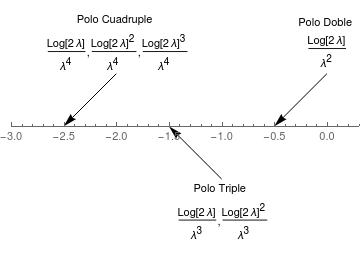
\includegraphics[scale=0.6]{Polos.jpg}
    \caption{En este caption se puede ver la contribucion a los polos generador por el termino $Log[
	\frac{\alpha c Log[2 \lambda] - \lambda f[\lambda] }{\Gamma \left[1 + \frac{i \alpha}{ 2 \lambda} \right] } + 
	c \alpha \Gamma \left[ - \frac{i \alpha}{2 \lambda} \right] ]$ }
    \label{fig:Dibujo}
\end{figure}

$\mathbf{
		Log[- \alpha c Log[2 \lambda] + \lambda f[\lambda] ]
		}: 
		$ \\

Al igual que con el termino en la rama anterior, voy a sacar factor comun $\lambda$ para que quede:

\begin{equation}
Log[\lambda] + 
Log[i c - \frac{\alpha c Log[2 \lambda] }{\lambda} + 
\sum _{n=1} ^{\infty} \frac{f _n}{\lambda ^{n+1}} ]
\end{equation}

Este termino tiene la misma forma que el anterior, haciando el mismo tratamiento obtengo:

\begin{equation}
\begin{array}{c}
Log[- \alpha c Log[2 \lambda] + \lambda f[\lambda] ] = \\
Log[\lambda] + Log[i c] + 
\sum _{m=0} ^{\infty} \frac{(-1)^{n+1}}{(i c) ^m m}
							\left(
								\sum _{p=0} ^{\infty} {m\choose p} 
									\left( - \frac{ \alpha c Log[2 \lambda] } {\lambda} \right) ^p
									\left( \sum _{n=1} ^{\infty} \frac{f _n}{\lambda ^n} \right) ^{m-p} 
								\right)
\end{array}
\end{equation}

Donde se puede ver el mismo la misma forma de contribucion a los polos 



Te recomiendo leer \cite{yo}
